\section{实验评估}
\label{sec:experiments}

我们在两个基准系统上评估所提出的转移证书合成方法，以展示其在形式化 LTL 验证中的有效性及其计算优势。我们与三个基线进行比较：状态三元组方法~\cite{wongpiromsarn2015automata}、闭包证书~\cite{murali2024closure} 和神经闭包证书~\cite{nadali2024neural}。对于第一个基准 Kuramoto 振子模型（覆盖一维和二维场景），我们针对指定的 LTL 性质验证系统。对于第二个基准双房间温度模型，我们通过合成转移证书来满足复杂 LTL 要求，展示了我们方法的通用性，并突出了其在处理多样时序规约时的互补优势。所有实验均在 Ubuntu 22.04.3 LTS（Intel i7-9750H，8 GB RAM）上进行。在候选生成阶段，Z3 处理多项式模板的约束优化，而神经网络模板使用 Adam 优化器（学习率 0.001，1000 次迭代）训练，以最小化损失函数。对于形式化验证，我们使用 dReal（精度 0.0001）处理 Kuramoto 振子模型中的超越 $\sin$ 函数，而温度模型则使用 Z3。

\subsection{Kuramoto 振子}
\subsubsection{一维系统}
% 系统介绍
第一个基准是 Kuramoto 振子系统，形式化定义为 $\mathfrak{S} = (\mathcal{X}, \mathcal{X}_0, f)$，其动力学改编自~\cite{anand2022small}。该系统运行在状态空间 $\mathcal{X} = [0, 2\pi]$ 内，并从初始区域 $\mathcal{X}_0 = [\frac{4\pi}{9}, \frac{5\pi}{9}]$ 出发。为评估 LTL 验证，我们在时序性质中指定不安全区域 $\mathcal{X}_u = [\frac{7\pi}{9}, \frac{8\pi}{9}]$。离散时间转移函数 $f$ 给定为：
\begin{align}
f(x) = x + t_s\Omega + t_s K \sin(-x) - 0.532 x^2 + 1.69,
\end{align}
其中 $x$ 表示振子相位。系统参数设置如下：采样时间 $t_s = 0.1$，固有频率 $\Omega = 0.01$，耦合强度 $K = 0.0006$。



% 如何将安全性验证转化为LTL验证
我们考虑定义在原子命题集合 $AP = \{a\}$ 上的 LTL 规约 $\phi = \mathbf{G}\neg a$，其标记函数定义为：当 $x \in \mathcal{X}_u$ 时 $\mathfrak{L}(x) = \{a\}$，否则 $\mathfrak{L}(x) = \emptyset$。否定规约 $\neg \phi = \mathbf{F} a$ 由图~\ref{pic-tbnba1} 所示的 NBA 刻画。该自动机包含从初始状态 $q_0 \in Acc^{\text{start}}$ 出发的接受转移 $(q_0, \emptyset, q_0)$ 和 $(q_0, \{a\}, q_0)$。

\begin{figure}[h]
  \centering
  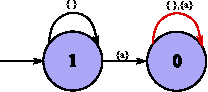
\includegraphics[width=0.3\textwidth]{pic/tbnba1-eps-converted-to.pdf}
  \caption{表示否定规约 $\mathbf{F} a$ 的 NBA。接受转移（以红色突出显示）描绘为状态 $q_0$ 上的自环。}
  \label{pic-tbnba1}
\end{figure}

% 多项式模板方法
基于转移安全性证书的定义，我们实现了一个基于多项式的 CEGIS 框架，用以合成保证指定 LTL 性质满足的证书。多项式模板结构如下：
\[
B_0(x, q; \mathbf{c}) = \sum_{i=0}^{4} c_i x^i + \sum_{j=1}^{3} c_{4+j} q^j + c_8 xq.
\]
合成过程首先从区域 $D_0$ 收集 30 个样本，从 $D_u$ 收集 600 个样本，并从 $D_{\mathcal{X}}$ 收集 1200 个样本。候选生成阶段被形式化为约束满足问题，并使用 Z3 求解器求解。由于系统动力学涉及超越 $\sin$ 函数，超出了 Z3 的判定过程范围，我们在验证阶段使用 dReal 求解器来识别反例。完整 CEGIS 循环在 1.76 秒内收敛，成功得到有效的转移证书：
\[
B_0(x, q) = -1 + 2q^2 - \frac{7}{16}xq.
\]

% 神经模板方法
除多项式模板外，我们还使用 CEGIS 框架合成神经转移证书 $B_0(x, q; \theta)$。该证书由一个 2-10-1 架构的前馈神经网络参数化，其中包含用于输入对 $(x, q)$ 的两个输入节点、具有 ReLU 激活的 10 个神经元隐藏层，以及单个线性输出。训练过程使用 250 个样本的数据集初始化（40 个来自 $D_0$，70 个来自 $D_u$，140 个来自 $D_{\mathcal{X}}$）。在每次迭代中，使用 dReal 求解器识别任何违反证书条件的点。随后将这些识别出的反例加入训练集，以逐步细化候选证书。完整 CEGIS 循环在 6.81 秒内收敛。过程中得到的有效证书见附录。

作为比较，状态三元组方法~\cite{wongpiromsarn2015automata} 在 0.10 秒内基于 4 次多项式模板为相关简单路径合成了屏障证书。证书 $B(x)=-4.5x^2+2x^3$ 通过状态三元组屏障条件阻断接受状态；其中一条接受边由于其标签区域为空而被平凡地处理。

\subsubsection{二维系统}

该基准进一步扩展到二维场景，其状态空间为 $\mathcal{X} = [0, \frac{8\pi}{9}]^2$，初始区域为 $\mathcal{X}_0 = [0, \frac{\pi}{9}]^2$。在这种情况下，不安全区域 $\mathcal{X}_u$ 被定义为状态空间的边界走廊：
\begin{equation}
\mathcal{X}_u = \left([0, \tfrac{8\pi}{9}] \times [\tfrac{5\pi}{6}, \tfrac{8\pi}{9}]\right) \cup \left([\tfrac{5\pi}{6}, \tfrac{8\pi}{9}] \times [0, \tfrac{8\pi}{9}]\right).
\end{equation}
耦合系统动力学 $f$ 由下式给出：
\begin{equation}
f(x_1, x_2) =
\begin{bmatrix} x_1 \\ x_2 \end{bmatrix}
+ t_s
\begin{bmatrix} \Omega + 1.69 \\ \Omega + 1.69 \end{bmatrix}
+ K t_s
\begin{bmatrix} \sin(x_2 - x_1) \\ \sin(x_1 - x_2) \end{bmatrix}
- 0.532 t_s
\begin{bmatrix} x_1^2 \\ x_2^2 \end{bmatrix}.
\end{equation}
为保持与一维分析一致，我们定义标记函数，使得当 $(x_1, x_2) \in \mathcal{X}_u$ 时 $\mathfrak{L}(x_1, x_2) = \{a\}$，否则为 $\emptyset$。验证针对相同的 LTL 规约 $\phi = \mathbf{G}\neg a$ 进行，并使用图~\ref{pic-tbnba1} 所示的 NBA。


对于二维系统，我们首先采用多项式模板 $B_0(x_1, x_2, q; \mathbf{c})$。合成过程使用的数据集包含来自 $D_0$ 的 30 个样本、来自 $D_u$ 的 729 个样本，以及来自 $D_{\mathcal{X}}$ 的 1,458 个样本。CEGIS 循环在 1.72 秒内生成有效转移证书：
\begin{equation}
B_0(x_1, x_2, q) = -1 + \tfrac{1}{8}x_1 x_2 + \tfrac{3}{2}q^2 - \tfrac{3}{32}q x_1^2 - \tfrac{153}{512}x_2 q.
\end{equation}
此外，我们实现了一个 3-15-1 架构的神经网络模板，其中包含用于元组 $(x_1, x_2, q)$ 的三个输入节点，以及具有 ReLU 激活的 15 个神经元隐藏层。为展示我们框架的效率，我们使用一组点初始化训练：40 个来自 $D_0$，90 个来自 $D_u$，180 个来自 $D_{\mathcal{X}}$。CEGIS 循环在 110.95 秒内收敛，并成功产生附录中的有效神经证书。

作为比较，状态三元组方法~\cite{wongpiromsarn2015automata} 在 1.13 秒内基于 2 次多项式模板为相关简单路径合成了屏障证书，得到 $B(x_1,x_2)=-x_1-x_2-3.125x_1x_2+2x_1^2+2x_2^2$。

\subsection{双房间温度}

第二个基准关注互连温度控制系统的形式化验证，记作 $\mathfrak{S} = (\mathcal{X}, \mathcal{X}_0, f)$，其动力学模型改编自~\cite{anand2024compositional}。该系统运行在状态空间 $\mathcal{X} = [20, 34]^2$ 内，并从初始配置 $\mathcal{X}_0 = [21, 24]^2$ 出发。底层 LTL 规约涉及目标区域 $\mathcal{X}_{VF} = [20, 26]^2$。具体地，系统状态演化由如下离散时间动力学 $f$ 控制：
\begin{equation}
f(x_1, x_2) = 
\begin{bmatrix} 1 - 2\alpha - \theta - \mu u(x_1) & \alpha \\ \alpha & 1 - 2\alpha - \theta - \mu u(x_2) \end{bmatrix}
\begin{bmatrix} x_1 \\ x_2 \end{bmatrix}
+ \mu T_h
\begin{bmatrix} u(x_1) \\ u(x_2) \end{bmatrix}
+ \theta
\begin{bmatrix} T_e \\ T_e \end{bmatrix},
\end{equation}
其中常数参数设为 $\alpha = 0.004$、$\theta = 0.01$、$\mu = 0.15$、$T_h = 40$ 和 $T_e = 0$。状态相关控制项定义为 $u(x_i) = 0.59 - 0.011 x_i$，其中 $i \in \{1, 2\}$。



考虑原子命题集合 $AP = \{a, b\}$，其中标记函数定义为：对于 $(x_1, x_2) \in \mathcal{X}_0$，有 $\mathfrak{L}(x_1, x_2) = \{a\}$；对于 $(x_1, x_2) \in \mathcal{X}_{VF}$，有 $b \in \mathfrak{L}(x_1, x_2)$。要求系统满足 LTL 规约 $\phi = a \Rightarrow \mathbf{FG}\neg b$。相应 NBA 捕获该规约的否定（即 $\neg \phi = a \land \mathbf{GF} b$），如图~\ref{pic-tbnba2} 所示。由于 $q_1$ 是唯一的接受转移起始状态，且初始区域 $\mathcal{X}_0 = [21,24]^2$ 被 $\mathfrak{L}$ 完全标记为 $\{a\}$，因此自动机从任意初始乘积状态出发都会在第一步转移到 $q_1$。这使得 $q_1$ 立即可达，因此无法为 $q_1$ 找到转移安全性证书。于是我们应用转移持久性证书来界定从 $q_1$ 出发的接受转移能够触发的次数。


\begin{figure}[h]
  \centering
  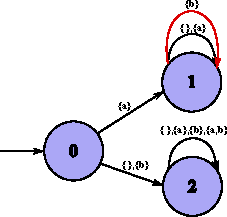
\includegraphics[width=0.3\textwidth]{pic/tbnba2-eps-converted-to.pdf}
  \caption{用于 $a \land \mathbf{GF} b$（$a \Rightarrow \mathbf{FG}\neg b$ 的否定）的 NBA。接受转移（红色）为 $(q_1, \{b\}, q_1)$ 和 $(q_1, \{a,b\}, q_1)$。}
  \label{pic-tbnba2}
\end{figure}

考虑转移持久性证书模板（见附录~\ref{appendix-experiment}）。我们为 $D_0$ 收集 16 个样本，为 $D_{\mathcal{X}}$ 收集 196 个样本。我们在 2.68 秒内得到有效的转移持久性证书 $$B_{1,1}(x_1, x_2) = 27 I_{[20,26]^2}(x_1, x_2) - x_1 I_{[20,26]^2}(x_1, x_2)$$ 以及 $\epsilon = 0.25$。

我们应用神经 CEGIS 来为 $Acc^{1,1}$ 合成 $B_{1,1}(x_1, x_2)$，使用架构为 2-3-1 的神经网络模板（2 个输入对应 $(x_1, x_2)$，3 个隐藏神经元采用平方激活，1 个输出）。我们为 $D_{\mathcal{X}}$ 收集 100 个样本，并为 $D_0$ 收集 16 个样本。整个 CEGIS 循环在 1461.91 秒内终止，所得有效证书见附录。

相比之下，状态三元组方法~\cite{wongpiromsarn2015automata} 在该基准上超时。由于初始区域完全包含在目标区域 $\mathcal{X}_{VF}$ 内，使得接受自动机状态可达，而状态三元组的路径阻断义务过于保守，因此在时间限制内无法通过屏障证书阻断接受路径。

\subsection{比较}
我们主要将本方法与状态三元组方法~\cite{wongpiromsarn2015automata} 和闭包证书~\cite{murali2024closure} 进行比较。状态三元组方法是一种基础的自动机理论方法，它构造屏障证书以阻断自动机中从初始状态到接受状态的所有简单路径，并要求枚举这些路径上的状态三元组。闭包证书专门用于提供比状态三元组方法更一般的验证条件，而神经闭包证书~\cite{nadali2024neural} 使用神经网络模板扩展了这一思想。双房间温度基准具体展示了相对于状态三元组方法的优势。NBA 包含从 $q_1$ 到 $q_1$ 的接受转移，其标签为 $\{b\}$ 和 $\{a,b\}$；由于标记函数将整个初始区域 $\mathcal{X}_0=[21,24]^2$ 映射为 $\{a\}$，自动机状态 $q_1$ 在进入乘积系统时立即可达。因此，状态三元组方法要求通过屏障证书阻断到接受状态的所有路径，而由于 $q_1$ 不可能变为不可达，该方法在结构上不适用，从而导致超时。我们的转移持久性证书 $B_{1,1}$ 通过界定接受转移能够触发的次数解决了这一问题，而无需要求 $q_1$ 不可达。闭包证书的核心思想在于刻画转移闭包的过近似，因此用于 LTL 验证的闭包证书定义在 $\mathcal{X} \times \mathcal{X} \times Q \times Q$ 上。相比之下，我们的方法采用转移安全性证书来直接过滤不可达自动机状态，或使用转移持久性证书来证明接受转移只发生有限多次，其中转移安全性证书定义在 $\mathcal{X} \times Q$ 上，而转移持久性证书仅定义在 $\mathcal{X}$ 上。这将有效证书域从闭包证书的 $\mathcal{X} \times \mathcal{X} \times Q \times Q$ 降至至多 $\mathcal{X} \times Q$，并提高了合成效率。对于神经模板，我们采用 CEGIS 框架，而神经闭包证书方法依赖采样和事后验证：在以给定密度 $\epsilon$ 和安全裕度 $\eta$ 对状态空间进行采样之后，该方法训练到损失收敛为零，然后进行事后验证以确定所合成的证书是否有效。

我们进行了两组比较：（1）多项式模板 CEGIS 与状态三元组方法和闭包证书比较；（2）神经模板 CEGIS 与神经闭包证书比较。详细实验配置见附录~\ref{appendix-experiment}。表~\ref{tab:results-poly} 和表~\ref{tab:results-neural} 总结了总计算时间，其中“超时”表示合成超过一小时。如表~\ref{tab:results-poly} 所示，当选择合适模板时，我们基于多项式模板的 CEGIS 方法在数秒内完成合成。状态三元组方法在两个 Kuramoto 基准上也表现良好（0.10 秒和 1.13 秒），成功为相关简单路径合成屏障证书。然而，由于接受自动机状态从初始区域可达，使得路径阻断义务在结构上无法满足，它在双房间温度基准上超时；我们的转移持久性证书通过切换到有限发生论证解决了这一问题，并在 2.68 秒内完成。相比之下，在给定模板下，闭包证书方法仅在一维情况下快速合成证书；对于其他使用原论文中报告模板的案例，该方法超时，这与原工作中报告的合成通常需要超过一小时的结果一致。值得注意的是，在一维 Kuramoto 案例中，闭包证书（0.37 秒）优于我们的转移证书（1.76 秒）。这一结果是可以预期的，因为当状态维度较低且自动机最小时，闭包证书的扩展搜索空间 $\mathcal{X} \times \mathcal{X} \times Q \times Q$ 仍然可处理，因此我们方法的搜索空间优势尚未体现。该案例中的时间差异可归因于两个因素。第一，我们的 CEGIS 循环在验证阶段调用 dReal 处理超越 $\sin$ 函数，相比纯代数求解器引入了额外延迟。第二，我们的转移证书使用定义在 $(x, q)$ 上的 4 次多项式模板，包含 10 个单项式，而闭包证书基线采用的是仅定义在 $\mathcal{X}$ 上的 2 次模板；模板复杂度差异是时间比较中的另一个混杂因素。我们遵循原闭包证书论文中报告的模板，以保持一致的实验设置。然而，随着状态维度增加，$|\mathcal{X} \times \mathcal{X}|$ 的二次增长使闭包证书合成在计算上不可行（两个二维基准均超时），而我们的转移证书扩展性更好。转移安全性证书定义在 $\mathcal{X} \times Q$ 上，持久性证书仅定义在 $\mathcal{X}$ 上。二者都显著小于闭包证书域 $\mathcal{X} \times \mathcal{X} \times Q \times Q$，其中持久性证书实现了最大的缩减。类似地，如表~\ref{tab:results-neural} 所示，神经网络模板 CEGIS 最多在约 24 分钟内完成（双房间温度基准为 1461.91 秒），这比多项式模板版本慢得多，但仍显著快于神经闭包证书基线，后者在所有基准上均超时。对于双房间温度系统，多项式合成（2.68 秒）与神经合成（1461.91 秒）之间的巨大差距是可以预期的，并反映了候选生成阶段的根本差异。多项式 CEGIS 将证书合成形式化为由 Z3 直接求解的代数约束满足问题，当证书具有紧凑多项式形式时，该方法非常高效。相反，神经 CEGIS 在每轮 CEGIS 中执行 1000 次梯度下降迭代来更新网络参数，与多项式方法相比显著增加了总计算时间。尽管存在这一开销，神经模板方法在无法构造合适多项式模板时仍有价值；三个基准的神经结果都能在一小时阈值内完成，证明了这一点。神经闭包证书方法由于采样密度高，表现出显著更长的训练时间，这一结果与原论文报告的约 4 到 5 小时验证时间一致。这些结果表明，转移证书相对于状态三元组、闭包证书和神经闭包证书基线都实现了显著加速。这些收益来自两个互补来源：与闭包证书相比搜索空间更小，以及能够在逐转移基础上在安全性和持久性证明策略之间选择，这比承诺单一策略的方法提供了更大的验证灵活性。

\begin{table}[t]
\centering
\caption{多项式模板方法的合成时间比较（秒）}
\label{tab:results-poly}
\begin{tabular}{lccc}
\hline
\textbf{基准} & \textbf{转移证书} & \textbf{状态三元组} & \textbf{闭包证书} \\
\hline
Kuramoto 一维 & 1.76 & 0.10 & 0.37 \\
Kuramoto 二维 & 1.72 & 1.13 & 超时 \\
双房间温度 & 2.68 & 超时 & 超时 \\
\hline
\end{tabular}
\end{table}
\begin{table}[t]
\centering
\caption{合成时间比较（秒）}
\label{tab:results-neural}
\begin{tabular}{lcc}
\hline
\textbf{基准} & \textbf{转移证书} & \textbf{神经闭包证书} \\
\hline
Kuramoto 一维 & 6.81 & 超时 \\
Kuramoto 二维 & 110.95 & 超时 \\
双房间温度 & 1461.91 & 超时 \\
\hline
\end{tabular}
\end{table}
